\section{Design Constraints from Urban Road Usage}

This chapter builds a bridge between pure efficiency modeling and real-world usability. It introduces constraints imposed by urban infrastructure, user expectations, and traffic behavior. We first explore the spatial pressures that incentivize narrow and light vehicles. Then, we derive performance requirements (e.g., power-to-weight, acceleration, braking) needed to fluidly integrate with existing traffic. Finally, introduce the sketch of the proposed design in light of theses criterion.

\subsection{Urban Space: Width, Distance, and Parking Constraints}

The geometric footprint of a vehicle has a disproportionate impact in dense cities. A wide vehicle not only occupies more road space but also demands larger safety margins from other road users, longer parking slots, and wider lanes. Reducing width allows for better road sharing, denser parking, and higher capacity utilization of limited urban infrastructure. Minimizing frontal width also directly contributes to aerodynamic efficiency. 

Beyond static width, the effective road space a vehicle occupies also depends on its longitudinal spacing, which is governed by the driver's reaction time and travel speed. At a cruising speed \(v\) and a reaction time \(\tau\), the effective longitudinal space required per vehicle (headway) is approximately:
\[
s_{\text{eff}} = v \cdot \tau + l
\]
where \(l\) is the vehicle length. For example, at 50\,km/h (\(13.9\,\text{m/s}\)) and a conservative reaction time of 1.5\,s, the spacing is:
\[
s_{\text{eff}} = 13.9 \cdot 1.5 + 4.5 \approx 25.35\,\text{m}
\]
This means that an average vehicle occupies over 25 times 1.7 m square meters of road space at 50 kmh, even before accounting for lateral gaps.

Parking further amplifies this inefficiency. A typical car requires a footprint of at least \(2.0 \times 5.0 = 10\,\text{m}^2\), not including maneuvering space. This imposes a high space burden in cities already constrained by building density and infrastructure.\\
In contrast, our proposed vehicle, being light enough to be lifted to a vertical position, could feasibly occupy as little as:
\[
\boxed{0.65 \times 1.0 = 0.65\,\text{m}^2}
\]
This represents a more than 15-fold reduction in static parking footprint compared to conventional vehicles.\\
ADD HERE DRAWING SHOWING VEHICLE SHELL AND VERTICAL STORAGE
\subsection{Speed, Power and Traffic Fluidity}

To integrate fluidly and safely into urban traffic, a vehicle must have sufficient power to:
\begin{itemize}
    \item Climb steep inclines (e.g., up to 15\% gradient).
    \item Accelerate at a pace comparable to surrounding traffic (typically 0.1--0.3\,g).
    \item Reach legal urban speed limits (up to 50-60\,km/h).
\end{itemize}

\noindent
We define the power-to-weight ratio (PWR) as:
\[
    \text{PWR} = \frac{P}{m} \quad \text{[W/kg]}
\]
where $P$ is the mechanical power available at the wheels, and $m$ is the total mass of the system (vehicle + payload + passenger).

\subsubsection*{Hill Climbing Requirement}

The minimum power to climb a slope of angle $\theta$ at constant velocity $v$ is:
\[
    P_{\text{slope}} = m g \sin(\theta)\,v
\]

\noindent
For a 250\,kg system on a 15\% slope ($\theta \approx 8.6^\circ$) at 50\,km/h:
\[
    P = 250\,\text{kg} \cdot 9.81\,\text{m/s}^2 \cdot 0.15 \cdot \frac{50}{3.6} \approx \mathbf{5.3\,kW}
\]
This corresponds to a required PWR of:
\[
    \text{PWR}_{\text{min}} = \frac{5\,300}{250} \approx \mathbf{21\,W/kg}
\]

It is worth noting that this value is based on a \emph{worst-case} scenario: climbing a sustained 15\% gradient at 50\,km/h at maximum weight. In practice, the vehicle will likely will be lighter and either a lower climbing speed or accepting a short-duration higher power draw could reduce the sustained power requirement. Additionally, real gradients are often less severe or shorter in length.

Nevertheless, even accounting for these factors, the required power density remains in the same order of magnitude. A value between 10-30\,W/kg is a reasonable target for lightweight urban vehicles aiming to maintain functional parity with traditional car in urban settings.

\subsubsection*{Acceleration with Traction and Power Limits}

Electric drivetrains offer the advantage of delivering near-instant peak torque and high short-duration power relative to their steady-state consumption. Empirically, a lightweight electric vehicle may draw 2-3 times more power during short bursts. For acceleration we will thus use 3 times the steady state power density required

We model vehicle acceleration using two regimes:
\begin{enumerate}
    \item \textbf{Traction-limited phase:} The vehicle accelerates at a constant rate up to the maximum grip-limited threshold (e.g., 1\,g).
    \item \textbf{Power-limited phase:} Beyond a certain speed, acceleration is constrained by available mechanical power and follows:
    \[
        a(v) = \frac{P}{m\,v}
    \]
\end{enumerate}
as the speed increase the impact is non negligeable
A suitable metric for evaluating responsiveness in traffic is the \textbf{speed threshold beyond which the vehicle can no longer sustain a given acceleration}. This is computed using:
\[
v = \frac{P}{m\,a}
\quad\Rightarrow\quad
v_{\text{limit}} [\mathrm{km/h}] = \frac{3.6 \cdot P}{m \cdot a}
\]

\noindent
\newpage

Based on the following data from figure \ref{fig:break_event}

\begin{figure}[h!]
    \centering
    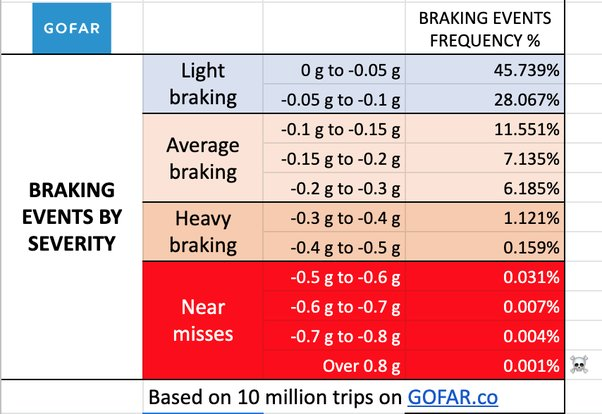
\includegraphics[width=0.5\linewidth]{Figures/ch3_gofarBrakingEvent.png}
    \caption{Real-World data about intensity and frequency of braking event from gofar.co\cite{noauthor_how_nodate}}
    \label{fig:break_event}
\end{figure}

we can deduce the following assuming that we tend to break harder or at least equally than we accelerate

\begin{itemize}
    \item \textbf{Comfortable acceleration:} Typically in the range of 0.2–0.3\,g ($\approx$ 2–3\,m/s²), especially in urban settings .
    \item \textbf{Comfortable braking:} Most braking events stay below 0.3\,g ($\approx$ 3\,m/s²), while emergency braking can exceed 0.7–0.9\,g briefly.
\end{itemize}


\vspace{1em}
\begin{table}[h!]
    \centering
    \renewcommand{\arraystretch}{1.3}
    \begin{tabularx}{\textwidth}{lcccccc}
        \toprule
        \textbf{Vehicle} & \textbf{Mass} & \textbf{Power} & \textbf{PWR} & \textbf{0.3\,g} & \textbf{0.5\,g} & \textbf{1.0\,g} \\
                         & [kg]         & [kW]           & [W/kg]       & [km/h]          & [km/h]          & [km/h] \\
        \midrule
        Tesla Model 3 (RWD)   & 1'745 & 211 & 121 & 148 & 89 & 44 \\
        Renault Zoe           & 1'502 & 100 & 67  & 81  & 49 & 24 \\
        Average compact car   & 1'300 & 66  & 51  & 62  & 37 & 19 \\
        Citroën 2CV           & 600    & 16  & 26.7  & 32.6  & 19.6 & 9.8 \\
        E-bike (pedal assist) & 100    & 0.25  & 2.5   & 3.1   & 1.8  & 0.9 \\
        \bottomrule
    \end{tabularx}
    \caption{Power-to-weight ratios and maximum speeds at which vehicles can sustain constant acceleration levels. Beyond these speeds, acceleration becomes power-limited.}
    \label{tab:accel_comfort_limits}
\end{table}

From this, we can infer that the power density required to be smooth in traffic should be between 25-40 W/kg peak to accomodate for acceleration as bellow would start to feel sluggish while higher will yield no benefit. One must keep in mind that the peak power density can be 2-3 times higher than the nomical power density for electric drive train and if we required 21 W/kg to be able to climb road we easily exceed 50 W/kg for acceleration.



\paragraph{Note on regenerative braking and battery design:}

While regenerative braking offers an opportunity to recover kinetic energy and improve overall efficiency, it is important to consider that it's often constrained by battery charge acceptance limits.

Standard lithium-ion battery packs can typically handle discharge rates up to 5\,C, but only accept charge rates of about 1\,C without degradation or overheating. This mismatch means that while high power can be drawn for acceleration, not all braking energy can be recovered at the same rate.

Furthermore, battery cell selection involves a trade-off: prioritizing power density (measured in W/kg) often comes at the expense of energy density (measured in Wh/kg). For regenerative braking to be effective, battery design must balance the need for peak power absorption with energy storage requirements.


\subsubsection*{Justifying Speed Limits}

Given a required peak power density of 25-40 W/kg and a steady state power density of 21 W/kg we can show that we can accomodate any speed found in an urban environment.

These power levels allow the vehicle to largely exceed typical city speed limits before aerodynamic drag becomes a limiting factor. For example, even with a modest power-to-weight ratio of just 10\,W/kg, a 250\,kg vehicle with optimized aerodynamics ($C_d = 0.15$, $A = 0.7$\,m²) and standard bike rolling resistance ($C_{rr} = 0.004$) can reach a steady-state cruising speed of:

\[
P_{\text{resist}}(v) = (\frac{1}{2} \rho C_d A v^2 + C_{rr} m g) v
\]

\[
v = \sqrt[3]{\frac{P}{\frac{1}{2} \rho C_d A + \frac{C_{rr} m g}{v^2}}} \quad \text{solved numerically} \quad \Rightarrow \boxed{116.6 \, \text{km/h}}
\]

This confirms that aerodynamic resistance is not a significant barrier below 80\,km/h for well-designed lightweight vehicles, and thus that power for acceleration will still be available at these speeds. From a safety standpoint, it is reasonable to cap the vehicle's maximum speed to 60-80\,km/h to reduce the severity of potential crashes and thus minimize the need for heavy structural reinforcements such as crumple zones. This design choice directly contributes to lower vehicle mass, further improving efficiency. On a safety standpoint it make sense to also cap the vehicule speed below 60-80 kmh to improve crash survivability and the reduce the need for crumple zone and security element which add weight. \\

One way to implement this whould be to limit the average power over a given time to match the average power from the user. On average, a person walking can generate 100-150 W. Assuming we compensate the losses and cancel out the energy spent accelerating or going uphill by the energy gained from decceleration and going downhill the previous equation whould show speed in 40-55 kmh range with the assumption that the vehicle is not fully loaded and thus only weight 150 kg yielding a Power density of 1W/kg. The second argument beyond being able to accomodate both terrain and traffic condition is that it provid a fairly strong incentive to keep the rider active which has been shown to have a positive health impact. The third argument in favor is that it would allow to legally consider the vehicle as a "cycle" according to the OETV\cite{noauthor_rs_nodate} which state the main difference between a cycle and the other category is the external energy to make the vehicle move. One could argue that as long as we only compensate loss using an external sources and average out the power by storing the user production then it's a "cycle".

\newpage

\subsection{Travel Time and Speed Requirements}

The marginal gain in travel time beyond 50\,km/h in cities is due to intersections, traffic lights, pedestrian crossings, and overall traffic congestion. To assess the impact of speed caps, we compare ideal and capped speed profiles for typical trips.

For most short trips ($<10$\,km), the difference between a capped vehicle (e.g., max 60\,km/h) and a conventional car (max 120\,km/h) is minimal, as higher speed segments are rare in urban settings. Empirical studies show that the median speed of urban car trips typically lies between 10 and 40\,km/h \cite{ma_real-world_2019}, indicating that speed caps do not meaningfully affect travel time in such contexts. Thus, the energy efficiency and safety benefits of capping the top speed far outweigh the negligible loss in time.

If greater precision is needed, we could directly use a Markov model of vehicle states parameterized by real-world measurements of driving regimes like it's done in the previously mentionned stufy to estimate time losses percentage from speed capping.
